\section{Motivation}
\label{sec:motivation}

Autonomous vehicles promise significant benefits to society, from reduced accident rates to greater mobility for the elderly. 
The biggest challenge in the design of autonomous vehicles comes from the uncertainty of the environment in which they will operate. 
Their control algorithms must be able to cope with driving events that occur on widely ranging time scales. 
For example, relaxed rural driving can accommodate planning actions every few seconds, while imminent collision avoidance requires planning and actuation on the order of a few milliseconds.
Thus `real-time' performance will imply different things depending on the context. 

A second, related, challenge is that the perception algorithms on-board these vehicles (like object detection based on video feed) must handle a very large amount of data, leading to increased power consumption. 
This is especially true for autonomous vehicles (AVs) since they carry multiple sensors (cameras, LIDAR, radars, ultrasound radars, etc) whose data must be processed in real-time to avoid accidents.

As a result of the variability in the environment, the control and perception systems are over-engineered to operate as if the worst-case conditions always hold. 
This results in unnecessarily high power consumption from the computation platform. It is worth noting that over the past few decades, the power consumption of processors has increased by more than double, while battery energy density has only improved by about a quarter \cite{Lahiri}. 

In the current work, we explore the idea of trading-off computation time and power for quality of output, and how this trade-off affects \emph{control performance}.
We start from the observation that the best quality output from the perception algorithm is not always required for the system to achieve the desired control performance.
For example, the control objective might be to follow the center of a driving lane, and control performance is measured by the deviation from that center.
At slow speeds, poor quality of position estimate may be tolerated since it won't lead to excessive deviations from the center.
Therefore we focus on \emph{anytime perception algorithms} that have a pre-defined set of interruption times. 
In general, the earlier the algorithm is interrupted, the worse is the quality of its output. 
On the other hand, that quality may be sufficient for the control algorithm to achieve its goal.

In \cite{RTSS15} we proposed a way in which a standard perception algorithm can be turned into an anytime algorithm via off-line profiling, and thus can offer a time/power/quality trade-off.
We also designed a model predictive controller than can make use of the trade-off offered by the anytime perception algorithm.
To achieve the time/power/quality trade-off, we produced multiple versions of the perception algorithm.
Broadly speaking, a version that ran for longer produced a higher quality output. 

In this work, we turn our attention to achieving the time/power/quality trade-off using \emph{platform-level} optimizations.
Specifically, we work with an autonomous car $1/10^{th}$ the size of a regular car (Fig. \ref{fig:traxxas}).
\begin{figure}[t]
	\centering
	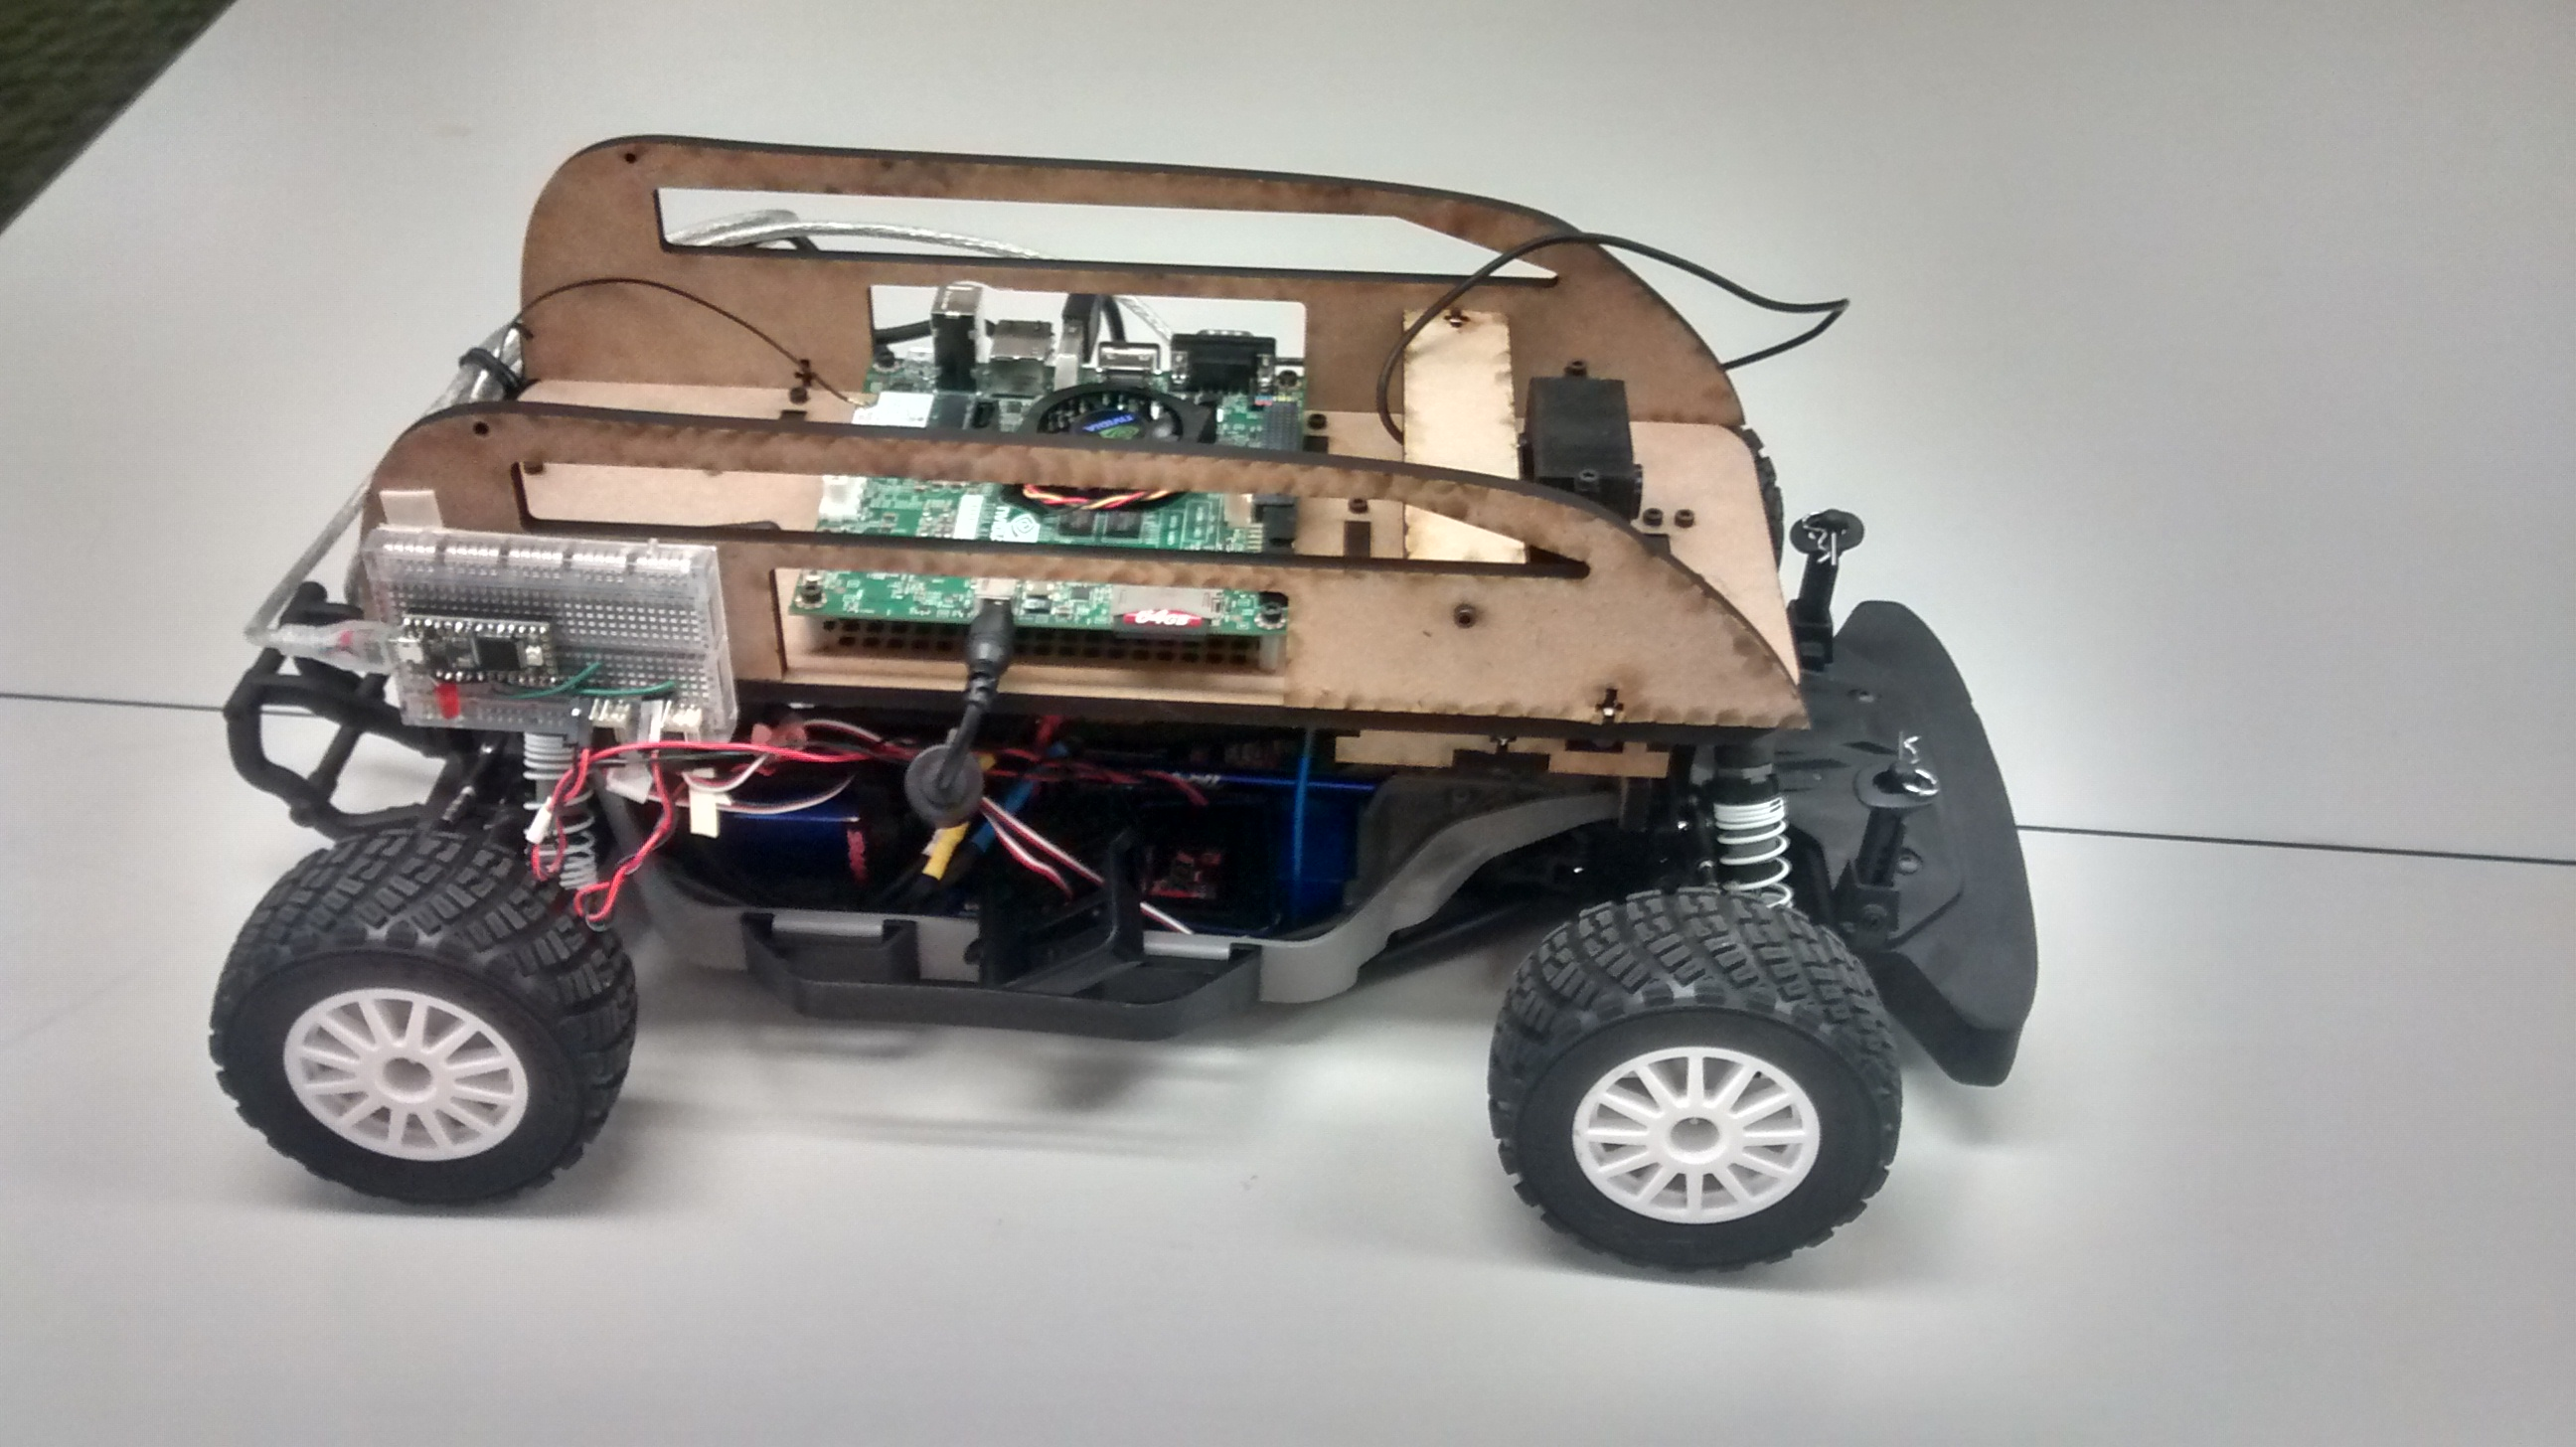
\includegraphics[scale=0.08]{traxxas.jpg}
	\caption{Traxxas autonomous car with camera.}
		\label{fig:traxxas}
\end{figure}  
It is equipped with a front facing monocular camera and runs the Vanishing Point perception algorithm \cite{VP1}. 
The on-board computation platform has both a CPU and GPU. More details of the experimental setup are in a later section.
The platform-level optimization divides the Vanishing Point algorithm into components, and decides whether to run each component on the CPU or GPU, and at what frequency.
The assignment to CPU or GPU is not static: every time the algorithm is executed, a different assignment may result, at a different frequency.
The assignment is dictated by the controller: based on off-line profiling of each processor's performance on each component, the controller decides what quality is currently acceptable while minimizing power consumption. The profiling is described in more detail in a later section.
In the present paper, we present initial results of partitioning the Vanishing Point algorithm and running different components on CPU and GPU, and at different frequencies.
We also provide the related power numbers, demonstrating that a meaningful difference in runtime and power consumption exists depending on the assignment and frequency.
In future work, we design a controller to make use of this and other optimizations, and relate the current results to the control performance.
%\todo[inline]{give example nb}
%
%
%Traditionally, perception algorithms were designed without consideration for the context in which their outputs will be produced
%Since the ultimaSince the meaning of real-time depends on the context, and 
%
%One impediment to achieving this real-time scalability variability 
%  presents In recent years, autonomous cars have become more and more prolific and increasingly capable \cite{}. For the perception and control software of these systems, there are stringent real-time requirements that have to be met for the safe performance of the system. In order for these requirements to be met, autonomous systems (both their hardware and software) are overengineered, resulting in a power consumption for the computation tasks that is not negligible. Also, while the focus of reducing power consumption in the design of such systems has been mostly on the power consumed by the actuators, computational platforms have been consuming more and more power. 
%It is worth noting that over the past few decades, the power consumption of processors has increased by more than double, while battery energy density has only improved by about a quarter [??Rajkumar??]. 
%
%In this poster, we present a method to obtain more energy efficient computations for the perception and estimation algorithms used in autonomous systems by exploiting hardware and algorithm level knobs. These knobs allow us to leverage a tradeoff between power consumption and a measure of quality of the perception and estimation algorithms. On-going work focuses also on coming up with a supervisory algorithm and control algorithms that are aware of this trade-off and choose an optimal operating point (or knobs settings) such that the performance of the overall closed-loop system is safe as well as energy efficient.
%
%Our method consists of a two-phase approach. The first involves extensively profiling the perception and estimation algorithm offline with all knob settings for timing, quality of output (if available) and power consumption. It also involves developing a control rule which chooses the best operating point for the perception and estimation algorithm while ideally providing mathematical guarantees on the safe performance of the system, e.g. as in \cite{} . The second, online stage, involves picking the best operating mode and control setting and run-time monitoring of the system performance. 
%
%We have developed an $1/10^{th}$ scale autonomous car testbed on which we evaluate our methods. In this particular work, we focus on a vanishing point algorithm based autonomous corridor navigation. We look at the algorithm level knobs, which are scheduling the sequential tasks of the vanishing point based algorithm on either the CPU or GPU; and the hardware level knobs which are frequencies of the CPU and GPU. Scheduling the tasks on different resources along with the different hardware settings result in a wide variety of timing and power distributions obtained.   
